\begin{figure}[h]\centering\caption{Impulse Response Function, Community Colleges, County Level}\begin{tabular}{cc}
\includegraphics[scale=0.6]{../tabfig/fig/cumresp_tef_tot47}&
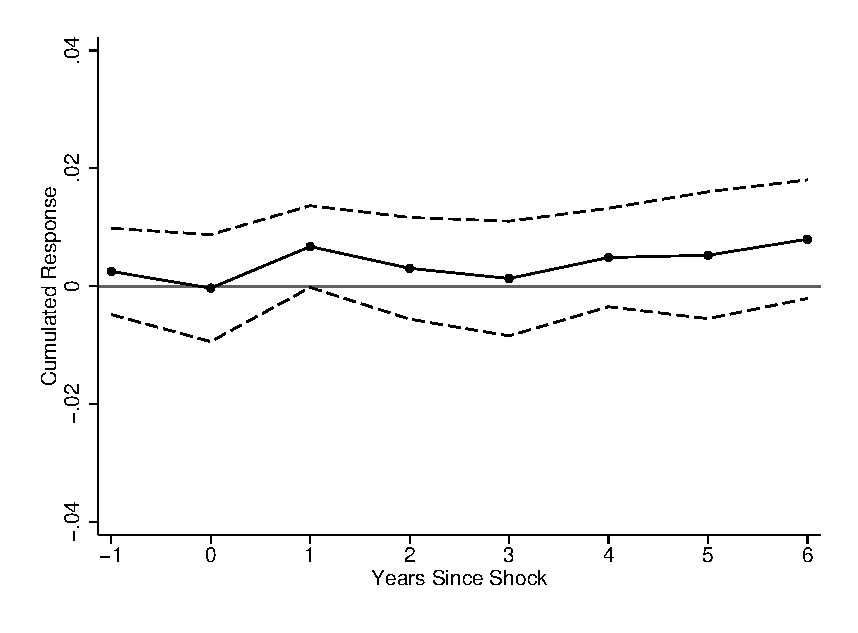
\includegraphics[scale=0.6]{../tabfig/fig/cumresp_aw_tot47}\\
(a) Fall Enrollment&(b) Total Awards\\
\includegraphics[scale=0.6]{../tabfig/fig/cumresp_aw_aa47}&
\includegraphics[scale=0.6]{../tabfig/fig/cumresp_aw_1t447}\\
(c) AA/AS Degrees&(d) 1-4 Year Certificates\\
\multicolumn{2}{p{6in}}{\footnotesize \emph{Notes:} Estimates are from Equation \ref{eqn:localproj}, where the outcome is the panel label, and the observation level is the county. The dotted lines are the 95\% confidence intervals.}
\end{tabular}
\label{fig:colproj}
\end{figure}



\begin{comment}
\begin{figure}[h]\centering
\caption{Completion Effects and Estimated Earnings Returns }
\begin{tabular}{c}
\includegraphics[scale=0.99]{../tabfig/fig/scatter_allwithcor.eps} \\
\multicolumn{1}{p{6in}}{\footnotesize \emph{Notes:} Estimated returns from \citet{SKG2014}. Each marker represents a two-digit CIP code field and award type (eg. AA/AS, 1-4 year certficate, $<$1 year certificate). The coefficient of the regression line is 4.39 (1.57).}
\end{tabular}
\label{fig:scatterall}
\end{figure}
\end{comment}



\clearpage
\begin{table}\caption{Broad Educational Categories}\scalebox{0.8}{
\begin{tabular}{lclc}
\hline\hline
Name	&	CIP Code	&		&	\# of Codes	\\\hline
Information Tech.	&	10	&	Communications Technologies/Technicians And Support Services.	&	15	\\
	&	11	&	Computer And Information Sciences And Support Services.	&	26	\\
    \hline
Construction/	&	15	&	Engineering Technologies/Technicians.	&	54	\\
Manufacturing	&	46	&	Construction Trades.	&	22	\\
	&	47	&	Mechanic And Repair Technologies/Technicians.	&	34	\\
	&	48	&	Precision Production.	&	16	\\
	&	49	&	Transportation And Materials Moving.	&	16	\\
    \hline
Public Services	&	43	&	Security And Protective Services.	&	16	\\
	&	44	&	Public Administration And Social Service Professions.	&	7	\\
    \hline
Health	&	51	&	Health Professions And Related Clinical Sciences.	&	196	\\\hline
Business	&	52	&	Business, Management, Marketing, And Related Support Services.	&	84	\\\hline
Family	&	19	&	Family And Consumer Sciences/Human Sciences.	&	32	\\\hline
Education	&	13	&	Edcuation	&	89	\\\hline
Personal	&	12	&	Personal And Culinary Services.	&	25	\\
\hline\hline
\end{tabular}}
\label{tab:cipapp}
\end{table}


\begin{table}[h]\centering\caption{Effect of Mass Layoffs on First-Time Fall Community College Enrollment Using Different Lags}\def\sym#1{\ifmmode^{#1}\else\(^{#1}\)\fi}\scalebox{0.8}{\begin{tabular}{lcccccc}
\hline\hline

& (1) & (2) & (3) & (4) & (5) &(6) \\
\hline
\input{../tabfig/lev/reg_incregmain_cz_ffe_tot_47}

\\\hline
Year FEs&X&X&X&X&X&X\\
CZ FEs&X&X&X&X&X&X\\
CZ Trends&X&X&X&X&X&\\
\hline\hline
\multicolumn{7}{p{5in}}{\footnotesize \emph{Notes:} Estimates are from equation \ref{eqn:main}, with different lag lengths. Outcome variable is total enrollment at community colleges in a commuting zone. All regressions include year and commuting zone fixed effects, commuting zone specific trends (except for column 6). Regressions are weighted by commuting zone population. Standard errors are clustered on commuting zone. *p$<$0.10, ** p$<$0.05, *** p$<$0.01}
\end{tabular}}
\label{tab:firstmain}
\end{table}




\begin{table}[h]\centering\caption{Mass Layoffs and Two-Year College Degrees and Certificates, by Program Type, Before and After 2007}
\def\sym#1{\ifmmode^{#1}\else\(^{#1}\)\fi}\scalebox{0.8}{\begin{tabular}{lK{2.2cm}K{2.2cm}K{2.2cm}K{2.2cm}K{2.2cm}K{2.2cm}K{2.2cm}}
\hline\hline
&Total&Career-Technical&Constr./ Manufac.&Health&IT&Public/ Protect.&Childcare/ Cosmet.\\
\hline\\

\multicolumn{6}{l}{\textbf{All Awards}}\\\input{../tabfig/lev/reg_prepost_fln_aw_tot_cz_justint}\hline\\
\multicolumn{6}{l}{\textbf{AA/AS}}\\\input{../tabfig/lev/reg_prepost_fln_aw_aa_cz_justint}\hline\\
\multicolumn{6}{l}{\textbf{1-4 Year Cert}}\\\input{../tabfig/lev/reg_prepost_fln_aw_1t4_cz_justint}\hline\\
\multicolumn{6}{l}{\textbf{$<$1 Year Cert}}\\\input{../tabfig/lev/reg_prepost_fln_aw_lt1y_cz_justint}\\


\hline\hline
\multicolumn{8}{p{8.2in}}{\footnotesize \emph{Notes:} Estimates are from equation \ref{eqn:main}. Outcome variables are total fall enrollment (panel A) and first-time fall enrollment (panel B) for demographic subgroups, listed at column head. All regressions include year and commuting zone fixed effects, commuting zone specific trends. Regressions are weighted by commuting zone population. Standard errors are clustered on commuting zone. *p<0.10, ** p<0.05, *** p<0.01}
\end{tabular}}
\label{tab:field_recession}
\end{table}




\begin{table}[h]\centering\caption{Mass Layoffs and Two-Year College Enrollment, Degrees and Certificates, County-Level Analysis}
\def\sym#1{\ifmmode^{#1}\else\(^{#1}\)\fi}\scalebox{0.8}{\begin{tabular}{lcccccccc}
\hline\hline
&(1)&(2)&(3)&(4)&(5)&(6)\\
&\multicolumn{2}{c}{Fall Enrollment}&\multicolumn{4}{c}{Associate's Degrees and Certificates}\\
&Total&First-Time&Total&AA/AS&1-4 Year Cert& $<$1 Year Cert\\
\hline\\

\input{../tabfig/lev/reg_mainregagg_47_cty}
\\
%\hline\\
%\multicolumn{4}{l}{\textbf{For-Profits}}\\
%\input{../tabfig/lev/reg_mainregagg_69_cty}\\\hline
Year FEs&X&X&X&X&X&X\\
County FEs&X&X&X&X&X&X\\
County Trends&X&X&X&X&X&X\\
\hline\hline
\multicolumn{7}{p{5.8in}}{\footnotesize \emph{Notes:} Estimates are from equation \ref{eqn:main}, but with observation level being the county rather than commuting zone. Outcome variables are listed at column head. All regressions include year and county fixed effects, county specific trends. Regressions are weighted by county population. Standard errors are clustered on commuting zone. *p$<$0.10, ** p$<$0.05, *** p$<$0.01}
\end{tabular}}
\label{tab:maincou}
\end{table}

\begin{comment}
\begin{table}[h]\centering\caption{Enrollment, Degrees and Certificates, Unweighted}
\def\sym#1{\ifmmode^{#1}\else\(^{#1}\)\fi}\scalebox{0.8}{\begin{tabular}{lcccccc}
\hline\hline
&(1)&(2)&(3)&(4)&(5)&(6)\\
&\multicolumn{2}{c}{Fall Enrollment}&\multicolumn{4}{c}{Associate's Degrees and Certificates}\\
&Total&First-Time&Total&AA/AS&1-4 Year Cert& $<$1 Year Cert\\
\hline\\

\input{../tabfig/lev/reg_mainregagg_47_cz_unwtre}
\\
%\hline\\
%\multicolumn{4}{l}{\textbf{For-Profits}}\\
%\input{../tabfig/lev/reg_mainregagg_69_cty}\\\hline
Year FEs&X&X&X&X&X&X\\
County FEs&X&X&X&X&X&X\\
County Trends&X&X&X&X&X&X\\
\hline\hline
\multicolumn{7}{p{6in}}{\footnotesize \emph{Notes:} Estimates are from equation \ref{eqn:main}, but with observation level being the county rather than commuting zone. Outcome variables are listed at column head. All regressions include year and county fixed effects, county specific trends. Standard errors are clustered on commuting zone. *p$<$0.10, ** p$<$0.05, *** p$<$0.01}
\end{tabular}}
\label{tab:mainunw}
\end{table}
\end{comment}


\begin{table}[h]\centering\caption{Enrollment, Heterogeneity by Gender and Race \label{tab:genderrace}}
\def\sym#1{\ifmmode^{#1}\else\(^{#1}\)\fi}
\scalebox{0.8}{
\begin{tabular}{lcccccccc}
\hline\hline
&(1)&(2)&(3)&(4)&(5)&(6)\\
&\multicolumn{2}{c}{\underline{Overall}}&\multicolumn{3}{c}{\underline{White and Asian}}&\multicolumn{3}{c}{\underline{Black, Hispanic, or Other Race}}\\
&Men&Women&Total&Men&Women&Total&Men&Women\\
\hline\\
\multicolumn{4}{l}{\textbf{Total Fall Enrollment}}\\
\input{../tabfig/lev/reg_mainregagg_47_cz_tef_heter}
\\\hline\\
\multicolumn{4}{l}{\textbf{First-Time Fall Enrollment}}\\
\input{../tabfig/lev/reg_mainregagg_47_cz_ffe_heter}
\\\hline
Year FEs&X&X&X&X&X&X&X&X\\
CZ FEs&X&X&X&X&X&X&X&X\\
CZ Trends&X&X&X&X&X&X&X&X\\
\hline\hline
\multicolumn{9}{p{7.2in}}{\footnotesize \emph{Notes:} Outcome variables are listed at the top of each column, and are the log counts of the corresponding outcome. Estimates are from equation \ref{eqn:main}. All regressions include year and commuting zone fixed effects, commuting zone specific trends. Standard errors are clustered on commuting zone. *p$<$0.10, ** p$<$0.05, *** p$<$0.01}
\end{tabular}}
\end{table}






\begin{table}[h]\centering\caption{Mass Layoffs and Two-Year College Enrollment, Degrees and Certificates, with Demographics}
\def\sym#1{\ifmmode^{#1}\else\(^{#1}\)\fi}\scalebox{0.8}{\begin{tabular}{lcccccc}
\hline\hline
&(1)&(2)&(3)&(4)&(5)&(6)\\
&\multicolumn{2}{c}{Fall Enrollment}&\multicolumn{4}{c}{Associate's Degrees and Certificates}\\
&Total&First-Time&Total&AA/AS&1-4 Year Cert& $<$1 Year Cert\\
\hline\\
\input{../tabfig/lev/reg_mainregagg_47_cz_xs}

Year FEs&X&X&X&X&X&X\\
CZ FEs&X&X&X&X&X&X\\
CZ Trends&X&X&X&X&X&X\\
\hline\hline
\multicolumn{7}{p{6in}}{\footnotesize \emph{Notes:} Outcome variables are listed at the top of each column, and are the log counts of the corresponding outcome. Estimates are from equation  \ref{eqn:main}. Panel (a) shows estimates for public community colleges, while panel (b) shows estimates for for-profit schools. All regressions include year and commuting zone fixed effects, commuting zone specific trends. Regressions are weighted by commuting zone population. Standard errors are clustered on commuting zone. *p$<$0.10, ** p$<$0.05, *** p$<$0.01}
\end{tabular}}
\label{tab:withdemogs}
\end{table}



%%%%%%%%%%%%%%%%%%%%%%%%%%%%%%%%%%%%%%%%%%%%%%%%%%%%%%%%%%%
\clearpage
\section{Local unemployment rates and educational production}
\label{sec:appunemp}
\doublespacing
A commonly used approach in the literature is to regress educational enrollment on the unemployment rate in the following way:

\begin{equation}
y_{ct}=\alpha+\beta U_{ct}+\Gamma X_{ct}+\gamma_c+\eta_t+\varepsilon_{ct}
\label{eq:ur}
\end{equation}
 where $y_{ct}$ is the logged value of a certain educational outcome and ${U_{ct}}$ is the local unemployment rate. The matrix $X_{ct}$ contains labor market covariates, $\gamma_c$ are local area fixed effects and $\eta_t$ are year fixed effects. This is a generalized form of the estimating equation in \citet{BF1995}. 
 
 There are, however, considerable concerns in explicitly estimating equation \ref{eq:ur}, though some variation of it is used with considerable frequency in the literature. First, enrollment in college mechanically increases the unemployment rate since those individuals are no longer counted as being in the labor force. Second, the unemployment rate, particularly at sub-state geographies, is measured with considerable error \citep{hoynes2000}, and therefore  would lead  $\beta$ to be biased towards zero. We discuss these issues in more depth in prior work \citep{FGS2015}.
 
 Table \ref{tab:umain} displays estimates of equation \ref{eq:ur} for the main outcomes. Although noisy, the coefficient in column 2 suggests that a one percentage point increase in the unemployment rate is associated with a 2.03 percentage point increase in first-time fall enrollment, which is roughly similar to the main result in \citet{BF1995}.


\begin{table}[h]\centering\caption{Unemployment Rate and Two-Year College Enrollment}
\def\sym#1{\ifmmode^{#1}\else\(^{#1}\)\fi}\scalebox{0.8}{\begin{tabular}{lcccccc}
\hline\hline
&(1)&(2)&(3)&(4)&(5)&(6)\\
&\multicolumn{2}{c}{Fall Enrollment}&\multicolumn{4}{c}{Associate's Degrees and Certificates }\\
&Total&First-Time&Total&AA/AS&1-4 Year Cert& $<$1 Year Cert\\
\hline\\
\input{../tabfig/lev/reg_urate1cz_47_cz}\\
Year FEs&X&X&X&X&X&X\\
CZ FEs&X&X&X&X&X&X\\
CZ Trends&X&X&X&X&X&X\\
\hline\hline
\multicolumn{7}{p{6in}}{\footnotesize \emph{Notes:} Outcome variables are listed at the top of each column, and are the log counts of the corresponding outcome. Estimates are from equation  \ref{eq:ur}. All regressions include year and commuting zone fixed effects, commuting zone specific trends. Regressions are weighted by commuting zone population. Standard errors are clustered on commuting zone. *p$<$0.10, ** p$<$0.05, *** p$<$0.01}
\end{tabular}}
\label{tab:umain}
\end{table}

